\documentclass[12pt]{article}
\usepackage[a4paper, margin=1in]{geometry}
\usepackage{amsmath}
\usepackage{amssymb}
\usepackage{amsthm}
\usepackage{amsfonts}
\usepackage{tabularx}
\usepackage{graphicx}
\newcounter{questionnumber}
\newenvironment{question}[1][]{\stepcounter{questionnumber}\par\noindent\textbf{Question \thequestionnumber. #1}\par}{\par}
\newenvironment{solution}{\par\noindent\textbf{Solution:}\par}{\par\vspace{1em}}
\begin{document}
\section{Discussion 03a}
\begin{question}
    You are at a party celebrating your completion of the CS 70 midterm. Show off your modular arithmetic skills and impress your friends by quickly figuring out the last digit(s) of each of the following numbers:\\
    (a) Find the last digit of $11^{3142}$.\\
    (b) Find the last digit of $9^{9999}$.\\
    (c) Find the last digit of $3^{641}$.
\end{question}
\begin{solution}
    \noindent
    (a) 1\\
    (b) 9\\
    (c) 3
\end{solution}
\begin{question}
    Prove or disprove the following statements:\\
    (a) There exists some $x \in \mathbb{Z}$ such that $x \equiv 3 \pmod{16}$ and $x \equiv 4 \pmod{6}$.\\
    (b) $2x \equiv 4 \pmod{12} \iff x \equiv 2 \pmod{12}$.\\
    (c) $2x \equiv 4 \pmod{12} \iff x \equiv 2 \pmod{6}$.
\end{question}
\begin{solution}
    \noindent
    (a) False. Assume that such an $x$ exists. Then $x \equiv 3 \pmod{16}$ means $x$ is odd and $x \equiv 4 \pmod{6}$ means $x$ is even, which leads to contradiction.\\
    (b) False. Consider $x=8$.\\
    (c) True. $2x \equiv 4 \pmod{12} \iff 2x=12k+4 \iff x=6k+2 \iff x \equiv 2 \pmod{6}$
\end{solution}
\begin{question}
    Recall the definition of inverses from lecture: let $a, m \in \mathbb{Z}$ and $m > 0$; if $x \in \mathbb{Z}$ satisfies $ax \equiv 1 \pmod{m}$, then we say $x$ is an inverse of $a$ modulo $m$.

    Now, we will investigate the existence and uniqueness of inverses.\\
    (a) Is 3 an inverse of 5 modulo 10?\\
    (b) Is 3 an inverse of 5 modulo 14?\\
    (c) For all $n \in \mathbb{N}$, is $3 + 14n$ an inverse of 5 modulo 14?\\
    (d) Does 4 have an inverse modulo 8?\\
    (e) Suppose $x, x' \in \mathbb{Z}$ are both inverses of $a$ modulo $m$. Is it possible that $x \not\equiv x' \pmod{m}$?
\end{question}
\begin{solution}
    \noindent
    (a) No. $3\times 5\equiv 5\left( \mathrm{mod}\;10 \right) $.\\
    (b) Yes. $3\times 5\equiv 1\left( \mathrm{mod}\;14 \right) $.\\
    (c) Yes. $\left( 3+14n \right) \times 5\equiv 3\times 5\equiv 1\left( \mathrm{mod}\;14 \right) $\\
    (d) No, since $\gcd(4,8)=4$.\\
    (e) No. $x\equiv xax' \equiv x' \left( \mathrm{mod}\;m \right) $.
\end{solution}
\begin{question}
    The Fibonacci sequence is given by $F_{n}=F_{n-1}+F_{n-2}$, where $F_{0}=0$ and $F_{1}=1$. Prove that, for all $n\geq1$,$\gcd(F_{n},F_{n-1})=1$.
\end{question}
\begin{solution}
    It is trivial for $n=1$. Assume that the statement holds true for all $n\leq k$.
    Then $\gcd(F_{k+1},F_k)=\gcd(F_{k+1}-F_k,F_k)=\gcd(F_{k-1},F_k)=1$.
    Therefore, the statement holds true for all positive integer $n$.
\end{solution}
\section{Discussion 03b}
\begin{question}
    In this problem, we will explore the Extended Euclid's Algorithm: first, the traditional implementation, and second, a faster, iterative version. Both ways yield the same result.

    Parts (b) and (c) explore the traditional Extended Euclid's Algorithm. The bolded numbers below keep track of which numbers appeared as inputs to the gcd call. Remember that we are interested in writing the GCD as a linear combination of the original inputs, so we don't want to accidentally simplify the expressions and eliminate the inputs.\\
    (a) As motivation, suppose we've found values of $a$ and $b$ such that $54a + 17b = 1$. With this knowledge, what is $17^{-1}$ (mod 54)?\\
    (b) Note that $x$ mod $y$, by definition, is always $x$ minus a multiple of $y$. So, in the execution of Euclid's algorithm, each newly introduced value can always be expressed as a ``combination'' of the previous two, like so:
    $$\begin{aligned}
    \gcd(54, 17) &= \gcd(17, 3) \\
    &= \gcd(3, 2) \\
    &= \gcd(2, 1) \\
    &= \gcd(1, 0) \\
    &= 1.
    \end{aligned}$$
    $$\begin{aligned}
    3 &= 1 \times 54 - 3 \times 17 \\
    2 &= 1 \times 17 - \_\_\_\_\times 3 \\
    1 &= 1 \times 3 - \_\_\_\_\times 2 \\
    [0 &= 1 \times 2 - \_\_\_\_\times 1]
    \end{aligned}$$
    (Fill in the blanks)\\
    (c) Recall that our goal is to fill out the blanks in
    $$1 = \_\_\_\times 54 + \_\_\_\times 17.$$
    To do so, we work back up from the bottom, and express the gcd above as a combination of the two arguments on each of the previous lines:
    $$
    1 = \_\_\_\times 3 + \_\_\_\times 2$$
    $$= \_\_\_\times 17 + \_\_\_\times 3$$
    $$
    = \_\_\_\times 54 + \_\_\_\times 17$$
    What does this imply, in this case, about the multiplicative inverse of 17, in arithmetic mod 54?\\
    (d) In the previous parts, we used a recursive method to write $\gcd(54, 17)$ as a linear combination of 54 and 17. We can also compute the same result iteratively - this is an alternative to the above method that is oftentimes faster. We begin by writing equations for our initial arguments, 54 and 17, as a linear combination of themselves:
    $$54 = 1 \times 54 + 0 \times 17$$
    $$
    17 = 0 \times 54 + 1 \times 17$$
    We can then use these initial equations (labeled $E_1$ and $E_2$ for ease of reference) to iteratively write reduced values as linear combinations of 54 and 17, until we are able to write an equation for gcd(54, 17), as desired.
    In particular, we want to subtract as many multiples of the second equation as possible from the first to create a new equation with a lower LHS value. We can keep iterating until the LHS becomes gcd(54, 17) = 1.
    $$\_\_\_ = \_\_\_ \times 54 + \_\_\_ \times 17 \quad (E_3 = E_1 - \_\_\_ \times E_2)$$
    $$
    \_\_\_ = \_\_\_ \times 54 + \_\_\_ \times 17 \quad (E_4 = E_2 - \_\_\_ \times E_3)$$
    $$1 = \_\_\_ \times 54 + \_\_\_ \times 17 \quad (E_5 = E_3 - \_\_\_ \times E_4)$$
    What does this imply, in this case, about the multiplicative inverse of 17, in arithmetic mod 54? Verify that your answer is equivalent to the previous part.\\
    (e) Calculate the gcd of 17 and 39, and determine how to express this as a ``combination'' of 17 and 39. What does this imply, in this case, about the multiplicative inverse of 17, in arithmetic mod 39?
\end{question}
\begin{solution}
    \noindent
    (a) $b \pmod{54}$\\
    (b) 5; 1; 2\\
    (c) 1; -1; -1; 6; 6; -19; The multiplicative inverse of 17 is 35 in arithmetic mod 54\\
    (d) 3; 1; -3; 3; 2; -5; 16; 5; 6; -19; 1; The multiplicative inverse of 17 is 35 in arithmetic mod 54\\
    (e) $\mathrm{gcd}\left( 39,17 \right) =1=7\times 39-16\times 17$. It implies that the multiplicative inverse of 17 is 23 in arithmetic mod 39.
\end{solution}
\begin{question}
    In this question, you will solve for a natural number $x$ such that,
    \begin{equation*}
    x \equiv 1 \pmod{3}
    \end{equation*}
    \begin{equation*}
    x \equiv 3 \pmod{7}
    \end{equation*}
    \begin{equation}
    x \equiv 4 \pmod{11}
    \end{equation}
    (a) Suppose you find 3 natural numbers $a, b, c$ that satisfy the following properties:
    \begin{equation}
    a \equiv 1 \pmod{3}; a \equiv 0 \pmod{7}; a \equiv 0 \pmod{11},
    \end{equation}
    \begin{equation}
    b \equiv 0 \pmod{3}; b \equiv 1 \pmod{7}; b \equiv 0 \pmod{11},
    \end{equation}
    \begin{equation}
    c \equiv 0 \pmod{3}; c \equiv 0 \pmod{7}; c \equiv 1 \pmod{11}.
    \end{equation}
    Show how you can use the knowledge of $a, b$ and $c$ to compute an $x$ that satisfies (1).
    In the following parts, you will compute natural numbers $a, b$ and $c$ that satisfy the above 3 conditions and use them to find an $x$ that satisfies (1).\\
    (b) Find a natural number $a$ that satisfies (2). That is, $a \equiv 1 \pmod{3}$ and is a multiple of 7 and 11. It may help to start with a number that is a multiple of both 7 and 11; what number should we multiply this by in order to make it equivalent to 1 (mod 3)?\\
    (c) Find a natural number $b$ that satisfies (3). That is, $b \equiv 1 \pmod{7}$ and is a multiple of 3 and 11.\\
    (d) Find a natural number $c$ that satisfies (4). That is, $c \equiv 1 \pmod{11}$ and is a multiple of 3 and 7.\\
    (e) Putting together your answers for parts (a), (b), (c) and (d), report an $x$ that satisfies (1).
\end{question}
\begin{solution}
    \noindent
    (a) $x=a+3b+4c$\\
    (b) $a=2\times 7\times 11=154$\\
    (c) $b=3\times 3\times 11=99$\\
    (d) $c=10\times 3\times 7=210$\\
    (e) $x=154=154+3\times 99+4\times 210=1291$
\end{solution}
\begin{question}
    Assume that $a$ does have a multiplicative inverse mod $m$. Let us prove that its multiplicative inverse can be written as $a^k \pmod{m}$ for some $k \geq 0$.\\
    (a) Consider the infinite sequence $a, a^2, a^3, \ldots \pmod{m}$. Prove that this sequence has repetitions.

    (\textbf{Hint}: Consider the Pigeonhole Principle.)\\
    (b) Assuming that $a^i \equiv a^j \pmod{m}$, where $i > j$, what is the value of $a^{i-j} \pmod{m}$?\\
    (c) Prove that the multiplicative inverse can be written as $a^k \pmod{m}$. What is $k$ in terms of $i$ and $j$?
\end{question}
\begin{solution}
    \noindent
    (a) Assume that the sequence has no repetition. The sequence has infinite terms but the there are only at most $m$ different numbers in modulo $m$ arithmetic, which leads to contradiction.\\
    (b) $a^{i-j}\cdot a^j\equiv a^i\left( \mathrm{mod}\;m \right) \Longrightarrow a^{i-j}\equiv 1\left( \mathrm{mod}\;m \right) $\\
    (c) $a^{i-j}\equiv 1\left( \mathrm{mod}\;m \right) \Longrightarrow a\cdot a^{i-j-1}\equiv 1\left( \mathrm{mod}\;m \right) \Longrightarrow k=i-j-1$
\end{solution}
\section{Homework 03}
\begin{question}
    Solve the following modular arithmetic equations for x and y.\\
    (a) $9x+5\equiv 7\pmod{13}$.\\
    (b) Show that $3x+12\equiv 4\pmod{21}$ does not have a solution.\\
    (c) The system of simultaneous equations $5x+4y\equiv 0\pmod{7}$ and $2x+y\equiv 4\pmod{7}$.\\
    (d) $13^{2023}\equiv x\pmod{12}$.\\
    (e) $7^{62}\equiv x\pmod{11}$.
\end{question}
\begin{solution}
    \noindent
    (a) $9x+5\equiv 7\left( \mathrm{mod}\;13 \right) \Longrightarrow 9x\equiv 2\left( \mathrm{mod}\;13 \right) \Longrightarrow x\equiv 2\times 3\equiv 6\left( \mathrm{mod}\;13 \right) $\\
    (b) $3x+12\equiv 4\left( \mathrm{mod}\;21 \right) \Longrightarrow 3x\equiv 13\left( \mathrm{mod}\;21 \right) \Longrightarrow x=\frac{21k+13}{3}=7k+\frac{13}{3}$, and there is no such integer $x$.\\
    (c) $3x\equiv 16\equiv 2\left( \mathrm{mod}\;7 \right) \Longrightarrow x\equiv 2\times 5\equiv 3\left( \mathrm{mod}\;7 \right) $, 
    $15+4y\equiv 1+4y\equiv 0\left( \mathrm{mod}\;7 \right) \Longrightarrow 4y\equiv 6\left( \mathrm{mod}\;7 \right) \Longrightarrow y\equiv 6\times 2\equiv 5\left( \mathrm{mod}\;7 \right) $\\
    (d) $x\equiv 13^{2023}\equiv 1^{2023}\equiv 1\left( \mathrm{mod}\;12 \right) $\\
    (e) $x\equiv 7^{62}\equiv 7^{60}\times 7^2\equiv 5\left( \mathrm{mod}\;11 \right) $
\end{solution}
\begin{question}
    \noindent
    (a) What is the multiplicative inverse of $n - 1$ modulo $n$? (Your answer should be an expression that may involve $n$)\\
    (b) What is the solution to the equation $3x \equiv 6 \pmod{17}$?\\
    (c) Let $R_0 = 0; R_1 = 2; R_n = 4R_{n-1} - 3R_{n-2}$ for $n \geq 2$. Is $R_n \equiv 2 \pmod{3}$ for $n \geq 1$? (True or False)\\
    (d) Given that $(7)(53) - m = 1$, what is the solution to $53x + 3 \equiv 10 \pmod{m}$? (Answer should be an expression that is interpreted $\pmod{m}$, and shouldn't consist of fractions.)
\end{question}
\begin{solution}
    \noindent
    (a) $n-1\pmod{n}$\\
    (b) $3x\equiv 6\left( \mathrm{mod}\;17 \right) \Longrightarrow x\equiv 6\times 6\equiv 2\left( \mathrm{mod}\;17 \right) $\\
    (c) True.\\
    (d) $53x\equiv 7\left( \mathrm{mod}\;m \right) \Longrightarrow x\equiv 7\times 7\equiv 49\left( \mathrm{mod}\;m \right) $
\end{solution}
\begin{question}
    Wilson's Theorem states the following is true if and only if $p$ is prime:
    \begin{equation*}
    (p-1)!\equiv-1\quad(\mathrm{mod~}p).
    \end{equation*}

    Prove both directions (it holds if AND only if $p$ is prime).

    Hint for the if direction: Consider rearranging the terms in $(p-1)!=1\cdot2\cdots\cdots(p-1)$ to pair up
    terms with their inverses, when possible. What terms are left unpaired?

    Hint for the only if direction: If $p$ is composite, then it has some prime factor $q.$ What can we say about $( p-1) !$ (mod $q) ?$
\end{question}
\begin{solution}
    If $p$ is prime, pair up terms with their inverses when possible, and only those terms whose inverse are themselves are left unpaired.
    If $x$ is left, then $x^2-1\equiv \left( \mathrm{mod}\;p \right) \Longrightarrow p\mid \left( x+1 \right) \land p\mid \left( x-1 \right) \Longrightarrow x=p-1\lor x=1\Longrightarrow \left( p-1 \right) !\equiv p-1\equiv -1\left( \mathrm{mod}\;p \right) $
    For the other direction, assume that $p$ is composite, then for any prime factor $q$, $\left( p-1 \right) !\equiv 0\left( \mathrm{mod}\;q \right) $, which means $q\mid \left( p-1 \right) !$.
    Since it holds true for every prime factor, it implies that $p\mid \left( p-1 \right) !$, which is contradictory with the condition.
    Therefore, $p$ must be prime.
\end{solution}
\section{Discussion 04a}
\begin{question}
    Consider an RSA scheme with modulus $N = pq$, where $p$ and $q$ are distinct prime numbers larger than 3.\\
    (a) What is wrong with using the exponent $e = 2$ in an RSA public key?\\
    (b) Recall that $e$ must be relatively prime to $p-1$ and $q-1$. Find a condition on $p$ and $q$ such that $e = 3$ is a valid exponent.\\
    (c) Now suppose that $p = 5$, $q = 17$, and $e = 3$. What is the public key?\\
    (d) What is the private key?\\
    (e) Alice wants to send a message $x = 10$ to Bob. What is the encrypted message $E(x)$ she sends using the public key?\\
    (f) Suppose Bob receives the message $y = 19$ from Alice. What equation would he use to decrypt the message? What is the decrypted message?
\end{question}
\begin{solution}
    \noindent
    (a) Since $p$ and $q$ are distinct prime numbers larger than 3, they are both odd, thus both $(p-1)$ and $(q-1)$ are even, which means they are surely divisible by 2.\\
    (b) Both $p$ and $q$ must be of the form $3k+2$ for some integer $k$.
    (c) $N=5\times 17=85, e=3$\\
    (d) $3d\equiv 1\left( \mathrm{mod}\;64 \right) \Longrightarrow d\equiv 43\left( \mathrm{mod}\;64 \right) $\\
    (e) $\mathrm{E}\left( x \right) \equiv 10^3\equiv 1000\equiv 65\left( \mathrm{mod}\;85 \right) $\\
    (f) $\mathrm{D}\left( y \right) \equiv 19^{43}\equiv 59\left( \mathrm{mod}\;85 \right) $
\end{solution}
\begin{question}
    Members of a secret society know a secret word. They transmit this secret word $x$ between each other many times, each time encrypting it with the RSA method. Eve, who is listening to all of their communications, notices that in all of the public keys they use, the exponent $e$ is the same. Therefore the public keys used look like $(N_1,e),\ldots,(N_k,e)$ where no two $N_i'$s are the same. Assume that the message is $x$ such that $0\leq x<N_i$ for every $i.$

    Further, in all of the subparts, you may assume that Eve knows the details of the modifed RSA schemes (i.e. Eve knows the format of the $N_i'$s, but not the specific values used to compute the $N_i'$s).\\
    (a) Suppose Eve sees the public keys $(p_1q_1,7)$ and $(p_1q_2,7)$ as well as the corresponding trans-
    missions. Can Eve use this knowledge to break the encryption? If so, how? Assume that Eve cannot compute prime factors efficiently. Think of $p_1,q_1,q_2$ as massive 1024-bit numbers. Assume $p_1,q_1,q_2$ are all distinct and are valid primes for RSA to be carried out.\\
    (b) The secret society has wised up to Eve and changed their choices of $N$,in addition to changing
    their word $x.$ Now, Eve sees keys $(p_1q_1,3),(p_2q_2,3)$, and $(p_3q_3,3)$ along with their transmissions. Argue why Eve cannot break the encryption in the same way as above. Assume $p_1,p_2,p_3,q_1,q_2,q_3$ are all distinct and are valid primes for RSA to be carried out.\\
    (c) Let's say the secret $x$ was not changed $(e=3)$,so they used the same public keys as before, but
    did not transmit different messages. How can Eve figure out $x?$
\end{question}
\begin{solution}
    \noindent
    (a) Eve can use the Euclidean Algorithm to compute $\gcd(p_1q_1, p_1q_2)=p_1$, and divide $p_1q_1$ and $p_1q_2$ by $p_1$, therefore he can easily compute the inverse of 7 and break the encryption.\\
    (b) Because the gcd of any 2 $N_i$'s is 1 and dividing it cannot give him any prime factor.\\
    (c) He can compute the multiplicative inverse of $p_1q_1p_2q_2$ in modulo $p_3q_3$ arithmetic and does the same to $p_2q_2$ and $p_3q_3$.
    Then, linearly combine $p_1q_1p_2q_2[(p_1q_1p_2q_2)^{-1}\pmod{p_3q_3}]$, $p_2q_2p_3q_3[(p_2q_2p_3q_3)^{-1}\pmod{p_1q_1}]$ and $p_1q_1p_3q_3[(p_1q_1p_3q_3)^{-1}\pmod{p_2q_2}]$ to figure out $x^3\pmod{p_1q_1p_2q_2p_3q_3}$.
    since $x<\min_{i}{N_i}<(p_1q_1p_2q_2p_3q_3)^{\frac{1}{3}}$, $x^3=x^3\pmod{p_1q_1p_2q_2p_3q_3}$ and he can figure out $x=x^{frac{1}{3}}$
\end{solution}
\begin{question}
    Alice wants to tell Bob her concert ticket number, $m$, which is an integer between 0 and 100 inclusive. She wants to tell Bob over an insecure channel that Eve can listen in on, but Alice does not want Eve to know her ticket number.\\
    (a) Bob announces his public key $(N = pq, e)$, where $N$ is large (512 bits). Alice encrypts her message using RSA. Eve sees the encrypted message, and figures out what Alice's ticket number is. How did she do it?\\
    (b) Alice decides to be a bit more elaborate. She picks a random number $r$ that is 256 bits long, so that it is too hard to guess. She encrypts that and sends it to Bob, and also computes $rm$, encrypts that, and sends it to Bob. Eve is aware of what Alice did, but does not know the value of $r$. How can she figure out $m$? (You may assume that $r$ is coprime to $N$.)
\end{question}
\begin{solution}
    \noindent
    (a) There is only 101 possible number so he can just try it all.\\
    (b) He can compute the multiplicative inverse of $r^e$ in module $N$ arithmetic and multiply it by $rm\pmod{N}$ to get $m^e$, and try all possible $m$ to get it.
\end{solution}
\section{Homework 04}
\begin{question}
    Mathematics and computing both owe an immense debt to textiles, where many key ideas originated.
    Instructions for knitting patterns will tell you to begin by ``casting on'' the needle some multiple of $m$ plus $r$, where $m$ is the number of stitches to create one repetition of the pattern and $r$ is the number of stitches needed for the two edges of the piece. For example, in the simple rib stitch pattern below, the repeating pattern is of length $m=4$, and you need $r=2$ stitches for the edges.\\
    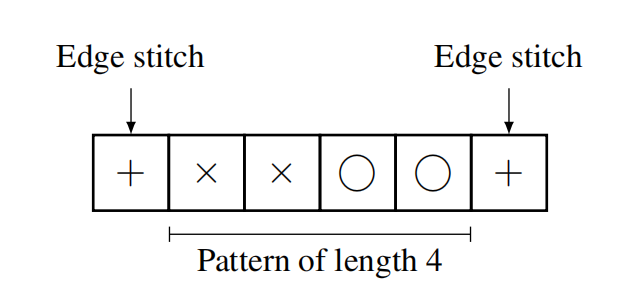
\includegraphics[width=0.5\textwidth]{graph1.png}

    Thus, to make the final piece wider, you can add as many multiples of the pattern of length 4 as you like; for example, if you want to repeat the pattern 3 times, you need to cast on a total of $3m+r=3(4)+2=14$ stitches (shown below).\\
    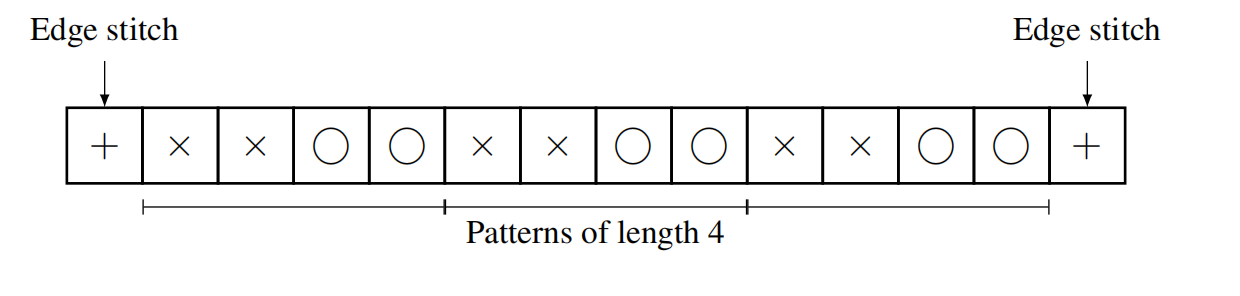
\includegraphics[width=0.5\textwidth]{graph2.png}

    You've decided to knit a 70-themed baby blanket as a gift for your cousin and want to incorporate rows from three different stitch patterns with the following requirements:
    \begin{itemize}
        \item Alternating Link: Multiple of 7, plus 4
        \item Double Broken Rib: Multiple of 4, plus 2
        \item Swag: Multiple of 5, plus 2
    \end{itemize}

    You want to be able to switch between knitting these different patterns without changing the number of stitches on the needle, so you must use a number of stitches that simultaneously meets the requirements of all three patterns.

    Find the smallest number of stitches you need to cast on in order to incorporate all three patterns in your baby blanket.
\end{question}
\begin{solution}
    $x=\left( 4\times 5\times 6\times 4+7\times 5\times 3\times 2+7\times 4\times 2\times 2 \right) \left( \mathrm{mod}\;140 \right) =102$
\end{solution}
\begin{question}
    Euler's Totient Theorem states that, if $n$ and $a$ are coprime,
    $$a^{\phi(n)} \equiv 1 \pmod{n}$$
    where $\phi(n)$ (known as Euler's Totient Function) is the number of positive integers less than or equal to $n$ which are coprime to $n$ (including 1). Note that this theorem generalizes Fermat's Little Theorem, since if $n$ is prime, then $\phi(n) = n - 1$.\\
    (a) Let the numbers less than $n$ which are coprime to $n$ be $m_1, m_2, \ldots, m_{\phi(n)}$. Argue that the set
    $$\{am_1, am_2, \ldots, am_{\phi(n)}\}$$
    is a permutation of the set
    $$\{m_1, m_2, \ldots, m_{\phi(n)}\}.$$
    In other words, prove that
    $$f : \{m_1, m_2, \ldots, m_{\phi(n)}\} \to \{m_1, m_2, \ldots, m_{\phi(n)}\}$$
    is a bijection, where $f(x) := ax \pmod{n}$.\\
    (b) Prove Euler's Theorem. (Hint: Recall the FLT proof.)
\end{question}
\begin{solution}
    \noindent
    (a) Assume that $am_i\equiv am_j\pmod{n}$ for some integer $i\neq j$.
    By definition, it means that $am_i-am_j=kn$ for some integer $k$.
    Since $a$ is coprime to $n$, it means that $m_i-m_j$ is divisible by $n$, which further implies that $m_i=m_j$, which leads to contradiction.
    Also, $a$ and $m_i$ are both coprime to $n$, which makes $am_i$ coprime to $n$.
    Therefore, f is a bijection.\\
    (b) According to (a), $a^{\phi \left( n \right)}m_1m_2...m_n\equiv m_1m_2...m_n\left( \mathrm{mod}\;n \right) \Longrightarrow a^{\phi \left( n \right)}\equiv 1\left( \mathrm{mod}\;n \right) $.
\end{solution}
\begin{question}
    A prime power is a number that can be written as $p^i$ for some prime $p$ and some positive integer $i.$
    So, 9= $3^2$ is a prime power, and so is 8= $2^3$. 42= 2$\cdot$3$\cdot$7 is not a prime power. 

    Prove that for any positive integer $k$, there exists $k$ consecutive positive integers such that none of
    them are prime powers.

    \textit{Hint: This is a Chinese Remainder Theorem problem. We want to find $n$ such that $(n+1),(n+2)$, $\ldots$, and $(n+k)$ are all not powers of primes. We can enforce this by saying that $n+1$ through $(n+k)$ each must have two distinct prime divisors. In your proof, you can choose these prime divisors arbitrarily.}
\end{question}
\begin{solution}
    Choose $2k$ prime numbers. List them as $p_1, p_2, \dots, p_2k(p_1<p_2<\dots<p_k)$
    Use Chinese Remainder Theorem to find a $n$ that for every $1\leq i\leq k$, $n\equiv -i\pmod{p_{2i-1}}$ and $n\equiv -i\pmod{p_{2i}}$.
    Therefore, for every $i$, $(n+i)$ must 2 distinct prime divisors $p_{2i-1}$ and $p_{2i}$.
\end{solution}
\begin{question}
    Consider the following RSA scheme and answer the specified questions.\\
    (a) Assume for an RSA scheme we pick 2 primes $p = 5$ and $q = 11$ with encryption key $e = 9$, what is the decryption key $d$? Calculate the exact value.\\
    (b) If the receiver gets 4, what was the original message?\\
    (c) Encode your answer from part (b) to check its correctness.
\end{question}
\begin{solution}
    \noindent
    (a) $9d\equiv 1\left( \mathrm{mod}\;40 \right) \Longrightarrow d\equiv 9\left( \mathrm{mod}\;40 \right) $\\
    (b) $4^9\equiv 14\left( \mathrm{mod}\;55 \right) $\\
    (c) $14^9\equiv 4\left( \mathrm{mod}\;55 \right) $
\end{solution}
\begin{question}
    You are trying to send a message to your friend, and as usual, Eve is trying to decipher what the message is. However, you get lazy, so you use $N = p$, and $p$ is prime. Similar to the original method, for any message $x \in \{0, 1, \ldots, N - 1\}$, $E(x) \equiv x^e \pmod{N}$, and $D(y) \equiv y^d \pmod{N}$.\\
    (a) Show how you choose $e$ and $d$ in the encryption and decryption function, respectively. Prove the correctness property: the message $x$ is recovered after it goes through your new encryption and decryption functions, $E(x)$ and $D(y)$.\\
    (b) Can Eve now compute $d$ in the decryption function? If so, by what algorithm?\\
    (c) Now you wonder if you can modify the RSA encryption method to work with three primes ($N = pqr$ where $p, q, r$ are all prime). Explain the modifications made to encryption and decryption and include a proof of correctness showing that $D(E(x)) = x$.
\end{question}
\begin{solution}
    \noindent
    (a) Find an $e$ that is coprime to $(p-1)$. Find the multiplicative inverse of $e$ in modulo $(n-1)$ arithmetic as $d$.
    By definition, $ed=k\left( p-1 \right) +1\Longrightarrow \mathrm{D}\left( \mathrm{E}\left( x \right) \right) \equiv m^{ed}\equiv \left( m^{\left( p-1 \right)} \right) ^k\cdot m\equiv m\left( \mathrm{mod}\;p \right) $.\\
    (b) Yes. By the extended Euclidean algorithm.\\
    (c) After modification, $e$ should be coprime to $(p-1)$, $(q-1)$ and $(r-1)$.
    Find a $d$ such that $ed\equiv 1\left( \mathrm{mod}\;\left( p-1 \right) \left( q-1 \right) \left( r-1 \right) \right) $.
    Then, by definition, $\mathrm{D}\left( \mathrm{E}\left( x \right) \right) \equiv m^{ed}\equiv m^{k\left( p-1 \right) \left( q-1 \right) \left( r-1 \right)}\cdot m\equiv m\left( \mathrm{mod}\;pqr \right) $.
\end{solution}
\end{document}